

\section{System Architecture}

\begin{figure}[ht!]
\centering
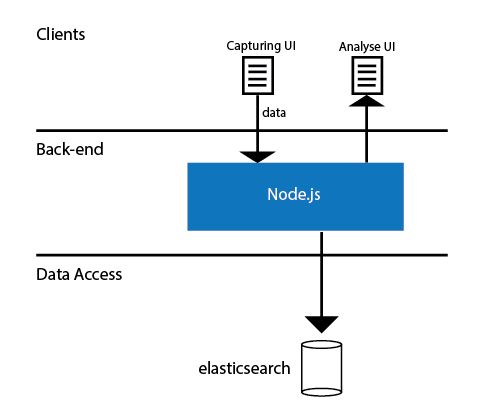
\includegraphics[width=100mm]{images/general/arhitecture.png}
\caption{}
\label{overflow}
\end{figure}

Client connects to the back-end web server via HTTP to request or insert information. There is two main interfaces; one for capturing new matches and attacks, and the second for analyse information. The back-end then again connects to an database to fetch or insert data. When fetching 

\subsection{Domain model}

The domain model is based around matches

{     
    "hometeam" : "Tromsø",
    "awayteam" : "Rosenborg",
    "score" : "1-0",
    "date" : '2013-15-09',
    "attacks": [
        {
            "time": 4,
            "touch" : 1,
            "team" : "Tromsø",
            "breakthrough" : "None",
            "breakthroughPlayer" : "None",
            "typeOfAttack" : "Dødball",
            "attackStart" : {
                "pos" : 17,
                "typeAction" : "Frispark",
                "player" : 403,
            },
            "passes": [
                {
                    "fromPlayer": 403,
                    "toPlayer": 393,
                    "fromPos": 17,
                    "toPos": 23,
                    "action": "CROSS"
                }
            ],
            "finish" : {
                "player": 393,
                "pos": 23,
                "action": "SHOTMISS"
            }
        },
}

\section{Implementation details}

\begin{table}[ht]
\caption{Software stack}
\begin{center}
\begin{tabular}{c|c}
    \hline
    \multicolumn{2}{c}{}\\
    Web server& Node.js\\
    Database& Elasticsearch\\
    Client & web  browser \\
\hline
\end{tabular}
\end{center}
\label{tab:multicol}
\end{table}


\subsection{Storage}

The data storage is an elasticsearch database. Elasticsearch is document oriented and works extremely well with JSON. As our server is built on JavaScript working with JSON is easy. JSON-objects can be inserted right into the storage and elasticsearch will map fields and value accordingly.  Our data input is generated in the web browser which also uses JavaScript and could have been inserted right away into the database without any pre mapping.
Elasticsearch takes advantages of embedded documents meaning we can store related data together. As an attack is usually made up of several passes you can store the passes as an embedded document inside the attack document so they can be retrieved in one query. 

The main reason for using Elasticsearch is its search capability. In a single query you can get counted how many passes all player for a team has played and received, number of times all players has been the breakthrough-player, type of attacks, most used zones for passing and finishing and so on. This makes it very easy and efficient to do queries for analyses on teams and players. After a query you can return all data directly to the client for him to expose to the end user.

\subsection{Back-end}

The back end is the middleware between the clients and the data layer. It exposes a RESTful interface over HTTP for the client to communicate. A request coming in is transformed to a database query based on the resource it tries to access. On answer from the database the result is transformed before returning it to the client. 

Similar if the client sends new data for a match the middle-ware inserts the data into the appropriate indexes.


\subsection{Front-end}

Front end is consist of a single page JavaScript application using Backbone.js as under-supporting framework. As it uses a MVC structure the models is responsible for AJAX communication with the back-end. 

For a analytic toolkit to be useful a good UI is critical. Here several helper library is used to present the data. Highcharts.js is JavaScript library for illustrating graphs. A query on team generates a lot of statistics and rather than listing them up they are presented using charts. This also gives us the advantage of displaying several numbers for each player and plot it in the same graph. In the image below we show the number of times a player has been involved in all attacks, number of passes into the final third of the pitch and the number of times a player has been the breakthrough-player.

\begin{figure}[ht!]
\centering
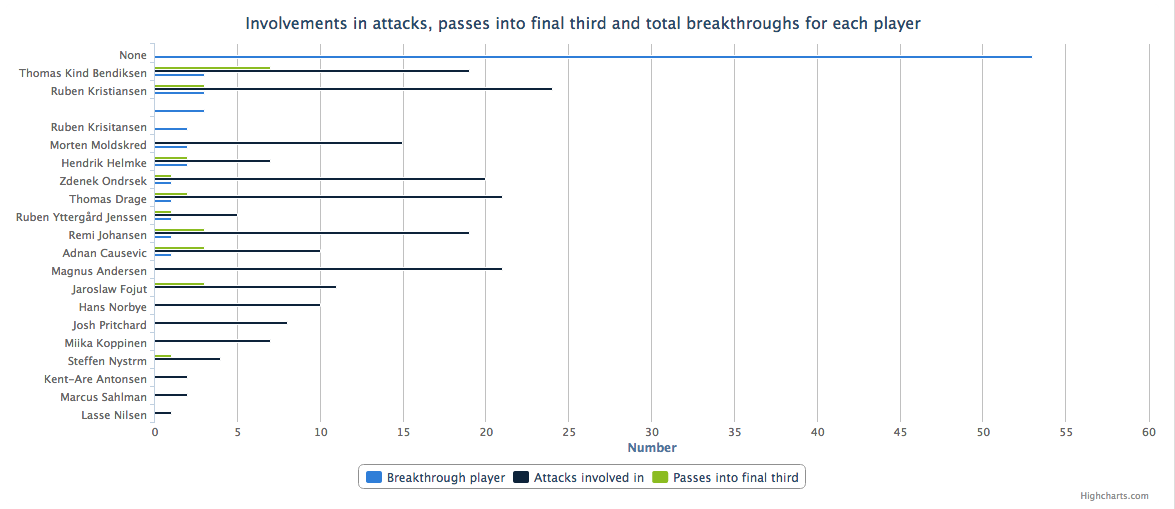
\includegraphics[width=100mm]{images/general/chart_passes.png}
\caption{Shows how the pass statistic is illustrated on the client by using Highcharts.js}
\label{overflow}
\end{figure}


Positional data is created using the a new feature of HTML5, canvases. From the model you get all zones with a number that symbols shots taken from that zone. This is then plotted into the respective zones. 

\begin{figure}[ht!]
\centering
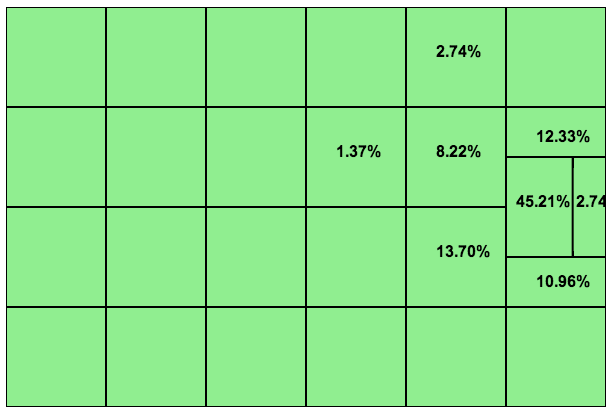
\includegraphics[width=85mm]{images/general/finishing_zones.png}
\caption{Illustrations of which zones the team has finished off their attacks from, with percent (team: Tromsø IL)}
\label{overflow}
\end{figure}

Backbone comes with a library Underscore.js that makes creating HTML pages with dynamic content easily. When you rending a new page on the site you can insert content retried from a model into the HTML and then render it.





\subsubsection{Security}
Secturity is not taken into convern. This means anyone getting into the page can post new match data. 